\documentclass[a4paper,11pt]{article}

\usepackage[T1]{fontenc}
\usepackage[utf8]{inputenc}
\usepackage{mathtools}
\usepackage[spanish,es-noquoting]{babel}
\usepackage{listings}
\usepackage[margin=1in]{geometry}
\usepackage{hyperref}
\usepackage{graphicx}
\usepackage{float}

\lstset{basicstyle=\small}
\newcommand{\shellcmd}[1]{\\\indent\indent\texttt{\footnotesize\$ #1}\\}

\begin{document}

\title{Final Programación Funcional}
\author{Strubolini Diego Martín}

\maketitle

\section{Introducción}

En el presente trabajo, se analizan distintas operaciones realizadas utilizando el modelo \textit{MapReduce}. Dichas operaciones pertenecen al dominio de las películas y se utilizan datos reales obtenidos del sitio \href{http://IMDb.com}{IMDb} en formato \textit{JSON}. El lenguaje de programación elegido es \textit{Haskell} y la librería elegida para la implementación del mencionado model es \textit{Haskell-MapReduce}.

Dicha implementación cuenta con la posibilidad de tener paralelismo al realizar las operaciones. Es por ello que se realizaron distintas pruebas con el objetivo de analizar el impacto de dicha característica.

\section{MapReduce}

\subsection{Principio Básicos}

El modelo de programación \textit{MapReduce} fue presentado por trabajadores de la empresa Google en el año 2008 \cite{dean2008mapreduce} como una solución sencilla a los procesamientos de gran escala dónde se require paralelismo y distribución.

El modelo comprende dos funciones claves:

La función \textit{map} o \textit{mapper} la cual procesa un entrada con clave/valor y produce una clave de salida y una valor intermedio:

\begin{lstlisting}
	map (in_key, in_value) -> list(out_key, intermediate_value)
\end{lstlisting}

La función \textit{reduce} o \textit{reducer} la cual combina todos los valores intermedios para una clave particular y produce un conjunto de valores agrupados:

\begin{lstlisting}
	reduce (out_key, list(intermediate_value)) -> list(out_value)
\end{lstlisting}

Dichas funciones están inspiradas en primitivas similares en LISP.

\subsection{Haskell MapReduce}

Este será el módulo a utilizar para el presente trabajo. La idea de implementar el modelo \textit{MapReduce} como una mónada fue presentado por Julian Porter en el año 2011 \cite{porter2011monad}.

Dicho módulo provee una interfaz de abstracción por sobre la implementación de dicha mónada lo que permite al usuario utilizar \textit{MapReduce} sin necesidad de conocer la implementación interna. 
\section{Módulos}

\subsection{IMDbMovie}

En este módulo se incluyen los tipos y los métodos que representan el dominio de una película. Para representar dicho tipo, se utilizó una estructura de registro con el objetivo de poder relacionar fácilmente los datos de los archivos \textit{JSON} con el tipo definido en Haskell de la siguiente manera:

\begin{lstlisting}[language=Haskell,frame=single]
data Movie = Movie { title      :: String
                   , year       :: String
                   , director   :: String
                   , genre      :: String
                   , imdbRating :: String
                   , imdbVotes  :: String
                   , product    :: String
                   , poster     :: String
                   , actors     :: String 
                   } deriving (Generic)
\end{lstlisting}

Se puede ver que todas los campos son de tipo \textit{String}, cuándo, por ejemplo, el año de una película tendría sentido que sea de algún tipo numérico. Es por esto, que se agregaron métodos en este módulo con el objetivo de obtener los datos de una película en un formato más conveniente.
Por ejemplo la función para obtener la calificación de una película:

\begin{lstlisting}[language=Haskell, frame=single]
imdbRatingNum :: Movie -> Float
imdbRatingNum movie = if (imdbRating movie) == "N/A" 
                      then 0 
                      else read (imdbRating movie) :: Float
\end{lstlisting}

También en este módulo se encuentran algunas operaciones simples sobre listas de películas, dónde se aprovechan varias funciones del lenguaje de manera que se expresen en una forma sencilla. Un ejemplo de esto, es la función obtener la película más votada de una lista de ellas.

\begin{lstlisting}[language=Haskell, frame=single]
topRated :: [Movie] -> [Movie]
topRated xs = filter (\m-> imdbRatingNum m == topRating) xs 
              where topRating = (maximum (map imdbRatingNum xs))
\end{lstlisting}

\subsection{JSONMovie}

El objetivo de este módulo es el de usar la librería \texttt{Data.Aeson} para poder leer los archivos en formato \textit{JSON} obtenidos del sitio \texttt{IMDb}.
Para poder realizar esto, se tuvieron que preprocesar los archivos con los datos de las películas por algunas restricciones del lenguaje. 

El principal problema fue que los campos dentro del tipo \texttt{Movie} (mostrado en la sección anterior), no pueden empezar con letra mayúscula, ya que sino es tomado como otro tipo. Es por esto que a todos los campos utilizados del archivo se les pasó la primer letra a minúscula. 

El segundo problema fue el tipo de cada elemento de la lista en el archivo. Dentro de los archivos hay información no sólo de películas, sino también de series, documentales, etc. Dicho campo que indicaba el tipo se llamaba \textit{type}, la cuál es otra es de las palabras reservadas para el lenguaje, por lo tanto se decidió cambiar su nombre a \textit{product}.

\subsection{MapReduceOperations}

Una vez conseguida la manera de representar la estructura de datos de una película y de cargarla con datos a partir de un archivo, ya se puede empezar a realizar operaciones sobre ella utilizando el modelo de MapReduce.
Dentro de este módulo, se encuentran todas las operaciones que se implementaron sobre una lista de películas utilizando el modelo previamente mencionado.

Para que la creación de dichos métodos sea más sencilla, se creó una función auxiliar llamada \texttt{MapReduce} la cual utilizarán todos los métodos como interfaz para acceder a los métodos provistos por la librería \texttt{Parallel.MapReduce.Simple}. 

\begin{lstlisting}[language=Haskell, frame=single]
mapReduce :: (Eq c, Binary a, NFData b, NFData c, NFData d1, NFData d2) 
                 => Int -> [a] -> ([a] -> [(b, c)]) -> ([b] -> [(d1, d2)])
                    -> [(d1,d2)]
mapReduce n state mapper reducer = run mr state
                                   where mr = distribute n >>= 
                                              lift mapper >>= 
                                              lift reducer 
\end{lstlisting}

Este método provee una capa de abstracción sobre el funcionamiento de dicha librería ya que logra que lo único que el desarrollador debe implementar es la función \textit{mapper} y \textit{reducer}, además de especificar la cantidad de mappers paralelos a utilizar.

Se puede destacar que la mayoría de los parámetros de dicha función son de tipo Binary o NFData, los cuales son necesarios ya que se cuenta con paralelismo. Dichos parámetros deben ser serializables con el objetivo de poder ser enviados entre distintos hilos de ejecución. También es entendible que el parámetro \texttt{c} tenga una función de igualdad ya que es necesaria para poder agrupar los resultados de los mappers en base a una misma clave.

Una vez definida dicha función, se implementaron las siguientes operaciones:

\begin{itemize}
	\item \textbf{topRatedMovie:} Películas más votadas agrupadas por el año de estreno. 
	\item \textbf{popularDirectors:} Directores cuya popularidad proviene de la suma de los votos de sus películas.
	\item \textbf{actorsCouple:} Películas en las cuales trabajaron juntos dos actores.
	\item \textbf{feticheActors:} Actores que trabajaron más veces junto a un director.
\end{itemize}

Algunas de dichas operaciones son más complejas que otras, pero tienen en común que, al utilizar el modelo MapReduce, son paralelizables.
\subsection{Main}

Módulo principal encargado de obtener los comandos ingresados por el usuario, llamar a las operaciones correspondientes e imprimir su resultado por consola. De acuerdo a la operación elegida, puede recibir parámetros adicionales con el objetivo de permitir una mayor flexibilidad al usuario a realizar operaciones en base a sus necesidades. Por ejemplo para cada una de las operaciones se puede especificar lo siguiente:

\begin{itemize}
	\item \textbf{topRatedMovie:} Año de las películas más votadas
	\item \textbf{popularDirectors:} Los N directores más populares
	\item \textbf{actorsCouple:} Actores que trabajaron juntos en N películas o más
	\item \textbf{feticheActors:} Actores que trabajaron más veces junto a un director específico.
\end{itemize}

\subsubsection{Compilación y Ejecución}
Para compilar el proyecto se deben compilar todos los módulos de la siguiente manera:
	\begin{lstlisting}[language=bash]
  $ ghc Main.hs IMDbMovie.hs JSONMovie.hs MapReduceOperations.hs -XDeriveGeneric
	\end{lstlisting}
  
El \texttt{-XDeriveGeneric} es necesario para poder derivar tipos genéricos. Una vez generado el ejecutable se lo puede utilizar de la siguiente manera:


  	\begin{lstlisting}[language=bash]
  $ ./Main <json_path> <operation_num> [operation_param] [num_mappers]
    \end{lstlisting}
    
\begin{itemize}
	\item \textbf{json\_path:} Path al archivo JSON.
	\item \textbf{operation\_num:} Número correspondiente a la operación que se desea realizar.
	\item \textbf{operation\_param:} Parámetro adicional para las operaciones
	\item \textbf{num\_mappers:} Cantidad de mappers a utilizar
\end{itemize}
  

\section{Paralelismo}

Para permitir que un programa escrito en haskell genere threads de ejecución se lo debe compilar con el flag \texttt{-threaded}. De esta manera, se habilita la generación de threads cuándo se utilizan estructuras de datos como \textit{parMap} del módulo \texttt{Control.Parallel.Strategies}. En el presente trabajo, el paralelismo es utilizado con el objetivo de distribuir las películas en distintos mappers con el objetivo de que actúen sobre distintos núcleos en la mayor medida posible.

Una vez logrado eso, se pueden ver los siguientes resultados obtenidos del tiempo de ejecución de algunas de las operaciones implementadas para distinta cantidad de núcleos y distinta cantidad de películas.


\subsection{Resultados}

Para cada operación se realizaron 5 corridas y se realizó el promedio del tiempo que demoró desde que se lo corre hasta que imprime el resultado.
Para obtener dicho valor se utilizó el comando \texttt{time} nativo de los sistemas \textit{BSD}. Las pruebas se realizaron utilizando de 1 a 4 cores o núcleos con el objetivo de comparar la performance para cada caso.

A continuación se muestran los resultados de las pruebas realizadas:

\begin{figure}[H]
    \centering
    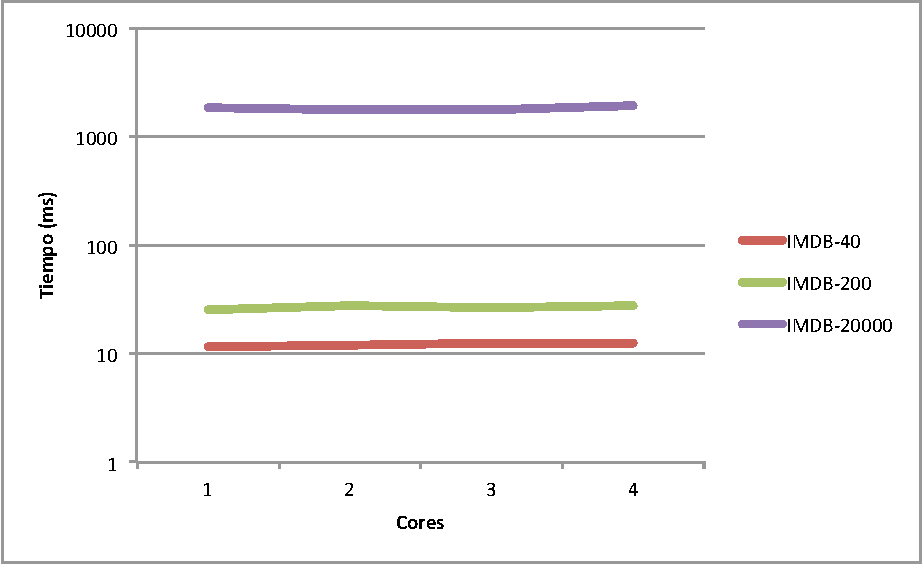
\includegraphics[width=0.75\textwidth]{images/topRated.pdf}
    \caption{Tiempo de ejecución del programa para la operación \texttt{topRated} para archivos de 40, 200 y 20000 películas}
    \label{fig:topRated}
\end{figure}

En la Figura \ref{fig:topRated} se puede ver dicha operación no fue afectada en gran medida por la utilización de varios cores. Esto se debe a que la operación \texttt{topRated} es la que requiere la menor cantidad de procesamiento de las operaciones implementadas. Por lo tanto, al agregar más núcleos, se indica que la información debe ser distribuida entre ellos y esto también afecta la performance. Al ser la operación que requiere menos procesamiento con respecto a las demás, es posible que no fuese necesario distribuir la información para la cantidad de registros de películas utilizada.

\begin{figure}[H]
    \centering
    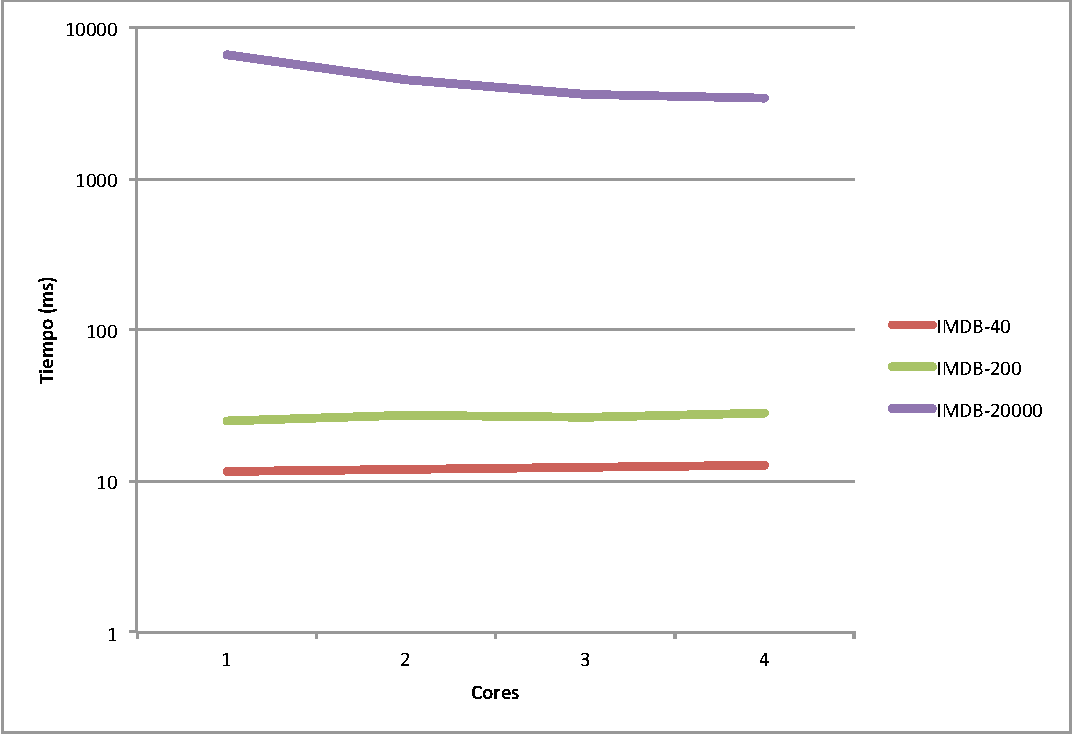
\includegraphics[width=0.75\textwidth]{images/popularDir.pdf}
    \caption{Tiempo de ejecución del programa para la operación \texttt{popularDirectors} para archivos de 40, 200 y 20000 películas}
    \label{fig:popDir}
\end{figure}

En la Figura \ref{fig:popDir} se puede ver un ejemplo donde para una gran cantidad de datos (20000 películas) se mejora la performance al distribuir el procesamiento entre distintos cores. Se puede ver que a medida que aumentan la cantidad de cores utilizados, se mejora el tiempo que demora el programa en devolver un resultado. Para los archivos con pocas películas, sucede lo mismo que en la operación anterior, es decir, no vale la pena distribuir dicho procesamiento si no se cuenta con una gran cantidad de datos.

\section{Conclusión}

El modelo \textit{MapReduce} resulta de gran utilidad cuándo se requiere analizar una gran cantidad de datos. Con solo aportar dos funciones, se pueden realizar operaciones que, acompañadas de la ventaja del lenguaje, logran escribirse de manera sencilla y además obtener resultados relevantes del dominio que se desea analizar.

Si se cuenta con un sistema distribuido, se puede ver una mejora en el tiempo de procesamiento cuándo se utilizan gran cantidad de datos a los cuales se les quiere realizar operaciones complejas.

\bibliographystyle{plain}
\bibliography{References}

\end{document}
